\documentclass[twoside]{book}

% Packages required by doxygen
\usepackage{calc}
\usepackage{doxygen}
\usepackage{graphicx}
\usepackage[utf8]{inputenc}
\usepackage{makeidx}
\usepackage{multicol}
\usepackage{multirow}
\usepackage{textcomp}
\usepackage[table]{xcolor}

% Font selection
\usepackage[T1]{fontenc}
\usepackage{mathptmx}
\usepackage[scaled=.90]{helvet}
\usepackage{courier}
\usepackage{amssymb}
\usepackage{sectsty}
\renewcommand{\familydefault}{\sfdefault}
\allsectionsfont{%
  \fontseries{bc}\selectfont%
  \color{darkgray}%
}
\renewcommand{\DoxyLabelFont}{%
  \fontseries{bc}\selectfont%
  \color{darkgray}%
}

% Page & text layout
\usepackage{geometry}
\geometry{%
  a4paper,%
  top=2.5cm,%
  bottom=2.5cm,%
  left=2.5cm,%
  right=2.5cm%
}
\tolerance=750
\hfuzz=15pt
\hbadness=750
\setlength{\emergencystretch}{15pt}
\setlength{\parindent}{0cm}
\setlength{\parskip}{0.2cm}
\makeatletter
\renewcommand{\paragraph}{%
  \@startsection{paragraph}{4}{0ex}{-1.0ex}{1.0ex}{%
    \normalfont\normalsize\bfseries\SS@parafont%
  }%
}
\renewcommand{\subparagraph}{%
  \@startsection{subparagraph}{5}{0ex}{-1.0ex}{1.0ex}{%
    \normalfont\normalsize\bfseries\SS@subparafont%
  }%
}
\makeatother

% Headers & footers
\usepackage{fancyhdr}
\pagestyle{fancyplain}
\fancyhead[LE]{\fancyplain{}{\bfseries\thepage}}
\fancyhead[CE]{\fancyplain{}{}}
\fancyhead[RE]{\fancyplain{}{\bfseries\leftmark}}
\fancyhead[LO]{\fancyplain{}{\bfseries\rightmark}}
\fancyhead[CO]{\fancyplain{}{}}
\fancyhead[RO]{\fancyplain{}{\bfseries\thepage}}
\fancyfoot[LE]{\fancyplain{}{}}
\fancyfoot[CE]{\fancyplain{}{}}
\fancyfoot[RE]{\fancyplain{}{\bfseries\scriptsize Generated on Sun Dec 6 2015 19\-:23\-:29 for Outletify by Doxygen }}
\fancyfoot[LO]{\fancyplain{}{\bfseries\scriptsize Generated on Sun Dec 6 2015 19\-:23\-:29 for Outletify by Doxygen }}
\fancyfoot[CO]{\fancyplain{}{}}
\fancyfoot[RO]{\fancyplain{}{}}
\renewcommand{\footrulewidth}{0.4pt}
\renewcommand{\chaptermark}[1]{%
  \markboth{#1}{}%
}
\renewcommand{\sectionmark}[1]{%
  \markright{\thesection\ #1}%
}

% Indices & bibliography
\usepackage{natbib}
\usepackage[titles]{tocloft}
\setcounter{tocdepth}{3}
\setcounter{secnumdepth}{5}
\makeindex

% Hyperlinks (required, but should be loaded last)
\usepackage{ifpdf}
\ifpdf
  \usepackage[pdftex,pagebackref=true]{hyperref}
\else
  \usepackage[ps2pdf,pagebackref=true]{hyperref}
\fi
\hypersetup{%
  colorlinks=true,%
  linkcolor=blue,%
  citecolor=blue,%
  unicode%
}

% Custom commands
\newcommand{\clearemptydoublepage}{%
  \newpage{\pagestyle{empty}\cleardoublepage}%
}


%===== C O N T E N T S =====

\begin{document}

% Titlepage & ToC
\hypersetup{pageanchor=false}
\pagenumbering{roman}
\begin{titlepage}
\vspace*{7cm}
\begin{center}%
{\Large Outletify }\\
\vspace*{1cm}
{\large Generated by Doxygen 1.8.6}\\
\vspace*{0.5cm}
{\small Sun Dec 6 2015 19:23:29}\\
\end{center}
\end{titlepage}
\clearemptydoublepage
\tableofcontents
\clearemptydoublepage
\pagenumbering{arabic}
\hypersetup{pageanchor=true}

%--- Begin generated contents ---
\chapter{u\-W\-S\-G\-I}
\label{md_server_README}
\hypertarget{md_server_README}{}
u\-W\-S\-G\-I can be used as both a web server and a python interface. Assuming our server will only have to deal with very light loads, this should be sufficient. If for whatever reason we decide we need a more standard web server, we could use something like nginx, but u\-W\-S\-G\-I would still be necessary as the python interface.

\subsection*{Installation}

There are packages for standard Linux distributions, but it's easier if we have a known, consistent starting point by building from source\-:

``` wget \href{http://projects.unbit.it/downloads/uwsgi-latest.tar.gz}{\tt http\-://projects.\-unbit.\-it/downloads/uwsgi-\/latest.\-tar.\-gz} tar xvzf uwsgi-\/latest.\-tar.\-gz cd $<$dir$>$ make ```

This will produce a uwsgi binary in the build directory -\/ this is the binary that will be referenced later.

\section*{Python}

Currently, the scripts assume Python 2 is used, though supporting 3 as well is trivial. We should decide on a version soon. \hyperlink{main_8py}{main.\-py} contains the function application, which is the entry point for the server. This is specified in the uwsgi invocation given below.

\subsection*{matplotlib and pyplot}

matplotlib includes pyplot, which seems to be useful for plotting stuff. In Ubuntu, the package python-\/matplotlib installs these Python modules.

\section*{The Database}

We all are at least somewhat familiar with S\-Q\-L now. I'd suggest using sqlite3, because the Python standard distribution provides an sqlite3 module, making setup very simple.

To create the test database\-: ``` python \hyperlink{create__db_8py}{create\-\_\-db.\-py} ```

To populate it with some random test data\-: ``` python \hyperlink{populate__test__db_8py}{populate\-\_\-test\-\_\-db.\-py} ```

\section*{Running the Server}

``` uwsgi --http \-:9090 --wsgi-\/file \hyperlink{main_8py}{main.\-py} --stats 127.\-0.\-0.\-1\-:9191 ``` The web server is listening on port 9090. In a browser, navigate to 127.\-0.\-0.\-1\-:9090. If all is well, you should see \char`\"{}\-Hello World\char`\"{}. Information about the running server can be found at 127.\-0.\-0.\-1\-:9191.

The server provides a very simple A\-P\-I that allows for creating and querying rows in test.\-db (in a very limited manner).

The H\-T\-M\-L template index.\-html is displayed by default. The page contains two forms\-: one for querying data and displaying a plot, and one for inserting new data into the database. Both forms use the A\-P\-I described below.

To create a new row, navigate to 127.\-0.\-0.\-1\-:9090/?insert=1\&id=$\ast$id$\ast$\&field=$\ast$field$\ast$, where {\itshape id} and {\itshape field} are an int and a string, respectively. For example, to insert a row with Id 2 and Field \char`\"{}fieldtwo\char`\"{}, navigate to 127.\-0.\-0.\-1\-:9090/?insert=1\&id=2\&field=fieldtwo. If it works, the bottom of the page should say \char`\"{}\-Inserted row\-: Id = 2, Field =
fieldtwo\char`\"{}.

To query a row by Id, navigate to 127.\-0.\-0.\-1\-:9090/?query=1\&id=$\ast$id$\ast$, where {\itshape id} is an int. If it works, the bottom of the page should display a plot of the current data for rows with an Id of {\itshape id}. 
\chapter{Sensor Interface}
\label{md_server_sensor_interface}
\hypertarget{md_server_sensor_interface}{}
Currently a sensor can log usage data by sending a post request to the root of the server where the body of the message is in json format. A message to log a single data point has the form\-: \begin{DoxyVerb}{
    "function": "insert",
    "timestamp": 0,
    "usage": 1
}
\end{DoxyVerb}


To log a point using curl\-: \begin{DoxyVerb}curl -X POST -d '{ "function": "insert", "timestamp": 0, "usage": 1 }' 127.0.0.1:9090\end{DoxyVerb}
 
\chapter{Outletify sensor}
\label{md_sensor_README}
\hypertarget{md_sensor_README}{}
\section*{Set up build environment}

\subsection*{Chibi\-O\-S}

Chibi\-O\-S is included as a git submodule. To download it, run\-: \begin{DoxyVerb}git submodule init
git submodule update
\end{DoxyVerb}


\subsection*{Toolchain}

T\-O\-D\-O\-: Add info

\subsection*{Programming}

On a aebian distro, run\-: \begin{DoxyVerb}sudo apt-get install dfu-util
\end{DoxyVerb}


T\-O\-D\-O\-: Add programming info 
\chapter{Namespace Index}
\section{Namespace List}
Here is a list of all documented namespaces with brief descriptions\-:\begin{DoxyCompactList}
\item\contentsline{section}{\hyperlink{namespacedb__interface}{db\-\_\-interface} \\*Provides a simple interface to an sqlite3 database configured for Outletify }{\pageref{namespacedb__interface}}{}
\item\contentsline{section}{\hyperlink{namespacemock__sensor}{mock\-\_\-sensor} \\*Mock sensor for testing the server }{\pageref{namespacemock__sensor}}{}
\item\contentsline{section}{\hyperlink{namespacemodels}{models} \\*Defines the class that makes up the relational database used for storing and visualizing the data }{\pageref{namespacemodels}}{}
\item\contentsline{section}{\hyperlink{namespaceplot}{plot} \\*Interface to pyplot for rendering Outletify data }{\pageref{namespaceplot}}{}
\item\contentsline{section}{\hyperlink{namespacerequest__handler}{request\-\_\-handler} \\*Parse request environments generated by uwsgi }{\pageref{namespacerequest__handler}}{}
\item\contentsline{section}{\hyperlink{namespacetests}{tests} \\*A simple test used to add an entry to the database and verify the output }{\pageref{namespacetests}}{}
\item\contentsline{section}{\hyperlink{namespaceurls}{urls} \\*Contains an array or url patterns to identify pages the server can display }{\pageref{namespaceurls}}{}
\item\contentsline{section}{\hyperlink{namespaceviews}{views} \\*Contains the functions required for building the pages defined in urls, reading and exporting the database }{\pageref{namespaceviews}}{}
\end{DoxyCompactList}

\chapter{Hierarchical Index}
\section{Class Hierarchy}
This inheritance list is sorted roughly, but not completely, alphabetically\-:\begin{DoxyCompactList}
\item Model\begin{DoxyCompactList}
\item \contentsline{section}{figure.\-models.\-Choice}{\pageref{classfigure_1_1models_1_1Choice}}{}
\item \contentsline{section}{figure.\-models.\-Usage}{\pageref{classfigure_1_1models_1_1Usage}}{}
\end{DoxyCompactList}
\item Test\-Case\begin{DoxyCompactList}
\item \contentsline{section}{figure.\-tests.\-Usage\-Test\-Case}{\pageref{classfigure_1_1tests_1_1UsageTestCase}}{}
\end{DoxyCompactList}
\end{DoxyCompactList}

\chapter{Class Index}
\section{Class List}
Here are the classes, structs, unions and interfaces with brief descriptions\-:\begin{DoxyCompactList}
\item\contentsline{section}{\hyperlink{classfigure_1_1models_1_1Choice}{figure.\-models.\-Choice} }{\pageref{classfigure_1_1models_1_1Choice}}{}
\item\contentsline{section}{\hyperlink{classfigure_1_1models_1_1Usage}{figure.\-models.\-Usage} }{\pageref{classfigure_1_1models_1_1Usage}}{}
\item\contentsline{section}{\hyperlink{classfigure_1_1tests_1_1UsageTestCase}{figure.\-tests.\-Usage\-Test\-Case} }{\pageref{classfigure_1_1tests_1_1UsageTestCase}}{}
\end{DoxyCompactList}

\chapter{File Index}
\section{File List}
Here is a list of all documented files with brief descriptions\-:\begin{DoxyCompactList}
\item\contentsline{section}{server/\hyperlink{create__db_8py}{create\-\_\-db.\-py} \\*Script to create an empty outletify power usage table }{\pageref{create__db_8py}}{}
\item\contentsline{section}{server/\hyperlink{dump__test__db_8py}{dump\-\_\-test\-\_\-db.\-py} \\*Script to print out the contents of 'outletify.\-db' }{\pageref{dump__test__db_8py}}{}
\item\contentsline{section}{server/\hyperlink{main_8py}{main.\-py} \\*Contains the entry point for the uwsgi server }{\pageref{main_8py}}{}
\item\contentsline{section}{server/\hyperlink{populate__test__db_8py}{populate\-\_\-test\-\_\-db.\-py} \\*Script to add some random data to an Outletify database }{\pageref{populate__test__db_8py}}{}
\end{DoxyCompactList}

\chapter{Namespace Documentation}
\hypertarget{namespacedb__interface}{\section{db\-\_\-interface Namespace Reference}
\label{namespacedb__interface}\index{db\-\_\-interface@{db\-\_\-interface}}
}


Provides a simple interface to an sqlite3 database configured for Outletify.  


\subsection*{Functions}
\begin{DoxyCompactItemize}
\item 
def \hyperlink{namespacedb__interface_a9dc663751479c6d0cec83e4895f65a43}{connect}
\item 
def \hyperlink{namespacedb__interface_a37ec95a825002d2d77c94c0f76512a0b}{close\-\_\-handle}
\item 
def \hyperlink{namespacedb__interface_a8e6ba6cc9f46178111842f698946c6fb}{create\-\_\-outletify\-\_\-tables}
\item 
def \hyperlink{namespacedb__interface_a03088d2791eade0146f7fd5bbc5926a0}{dump\-\_\-contents}
\item 
def \hyperlink{namespacedb__interface_ab7a5ac2ffbd107cc2f0a5745efd8c65c}{add\-\_\-row}
\item 
def \hyperlink{namespacedb__interface_a98ea80b49a8a41bffaecfb374b007abd}{query\-\_\-by\-\_\-timestamp}
\end{DoxyCompactItemize}
\subsection*{Variables}
\begin{DoxyCompactItemize}
\item 
\hypertarget{namespacedb__interface_a24d07298c20425fbb8b12f569270582c}{string {\bfseries D\-B\-\_\-\-N\-A\-M\-E} = 'outletify.\-db'}\label{namespacedb__interface_a24d07298c20425fbb8b12f569270582c}

\end{DoxyCompactItemize}


\subsection{Detailed Description}
Provides a simple interface to an sqlite3 database configured for Outletify. 

\subsection{Function Documentation}
\hypertarget{namespacedb__interface_ab7a5ac2ffbd107cc2f0a5745efd8c65c}{\index{db\-\_\-interface@{db\-\_\-interface}!add\-\_\-row@{add\-\_\-row}}
\index{add\-\_\-row@{add\-\_\-row}!db_interface@{db\-\_\-interface}}
\subsubsection[{add\-\_\-row}]{\setlength{\rightskip}{0pt plus 5cm}def db\-\_\-interface.\-add\-\_\-row (
\begin{DoxyParamCaption}
\item[{}]{timestamp, }
\item[{}]{usage, }
\item[{}]{dbhandle = {\ttfamily None}}
\end{DoxyParamCaption}
)}}\label{namespacedb__interface_ab7a5ac2ffbd107cc2f0a5745efd8c65c}

\begin{DoxyParams}{Parameters}
{\em dbhandle} & database handle from connect. Default database if None \\
\hline
{\em timestamp} & A timestamp value that can be converted to an int \\
\hline
{\em usage} & A usage value that can be converted to an int\\
\hline
\end{DoxyParams}
Adds a row to the given Outletify database \hypertarget{namespacedb__interface_a37ec95a825002d2d77c94c0f76512a0b}{\index{db\-\_\-interface@{db\-\_\-interface}!close\-\_\-handle@{close\-\_\-handle}}
\index{close\-\_\-handle@{close\-\_\-handle}!db_interface@{db\-\_\-interface}}
\subsubsection[{close\-\_\-handle}]{\setlength{\rightskip}{0pt plus 5cm}def db\-\_\-interface.\-close\-\_\-handle (
\begin{DoxyParamCaption}
\item[{}]{dbhandle}
\end{DoxyParamCaption}
)}}\label{namespacedb__interface_a37ec95a825002d2d77c94c0f76512a0b}

\begin{DoxyParams}{Parameters}
{\em dbhandle} & database handle from connect \\
\hline
\end{DoxyParams}
\hypertarget{namespacedb__interface_a9dc663751479c6d0cec83e4895f65a43}{\index{db\-\_\-interface@{db\-\_\-interface}!connect@{connect}}
\index{connect@{connect}!db_interface@{db\-\_\-interface}}
\subsubsection[{connect}]{\setlength{\rightskip}{0pt plus 5cm}def db\-\_\-interface.\-connect (
\begin{DoxyParamCaption}
\item[{}]{name = {\ttfamily DB\-\_\-NAME}}
\end{DoxyParamCaption}
)}}\label{namespacedb__interface_a9dc663751479c6d0cec83e4895f65a43}

\begin{DoxyParams}{Parameters}
{\em name} & The name of a database to connect to. Default to \char`\"{}outletify.\-db\char`\"{} \\
\hline
\end{DoxyParams}
\begin{DoxyReturn}{Returns}
Tuple containing a connection and cursor for the connection, used as a dbhandle for other methods in the module
\end{DoxyReturn}
Connects to an sqlite3 database \hypertarget{namespacedb__interface_a8e6ba6cc9f46178111842f698946c6fb}{\index{db\-\_\-interface@{db\-\_\-interface}!create\-\_\-outletify\-\_\-tables@{create\-\_\-outletify\-\_\-tables}}
\index{create\-\_\-outletify\-\_\-tables@{create\-\_\-outletify\-\_\-tables}!db_interface@{db\-\_\-interface}}
\subsubsection[{create\-\_\-outletify\-\_\-tables}]{\setlength{\rightskip}{0pt plus 5cm}def db\-\_\-interface.\-create\-\_\-outletify\-\_\-tables (
\begin{DoxyParamCaption}
\item[{}]{dbhandle = {\ttfamily None}}
\end{DoxyParamCaption}
)}}\label{namespacedb__interface_a8e6ba6cc9f46178111842f698946c6fb}

\begin{DoxyParams}{Parameters}
{\em dbhandle} & database handle from connect. Default database if None\\
\hline
\end{DoxyParams}
Creates a table named 'usage\-\_\-stats' with integer rows named 'timestamp' and 'usage' \hypertarget{namespacedb__interface_a03088d2791eade0146f7fd5bbc5926a0}{\index{db\-\_\-interface@{db\-\_\-interface}!dump\-\_\-contents@{dump\-\_\-contents}}
\index{dump\-\_\-contents@{dump\-\_\-contents}!db_interface@{db\-\_\-interface}}
\subsubsection[{dump\-\_\-contents}]{\setlength{\rightskip}{0pt plus 5cm}def db\-\_\-interface.\-dump\-\_\-contents (
\begin{DoxyParamCaption}
\item[{}]{dbhandle = {\ttfamily None}}
\end{DoxyParamCaption}
)}}\label{namespacedb__interface_a03088d2791eade0146f7fd5bbc5926a0}

\begin{DoxyParams}{Parameters}
{\em dbhandle} & database handle from connect. Default database if None \\
\hline
\end{DoxyParams}
\begin{DoxyReturn}{Returns}
An array describing the entire contents of the given database 
\end{DoxyReturn}
\hypertarget{namespacedb__interface_a98ea80b49a8a41bffaecfb374b007abd}{\index{db\-\_\-interface@{db\-\_\-interface}!query\-\_\-by\-\_\-timestamp@{query\-\_\-by\-\_\-timestamp}}
\index{query\-\_\-by\-\_\-timestamp@{query\-\_\-by\-\_\-timestamp}!db_interface@{db\-\_\-interface}}
\subsubsection[{query\-\_\-by\-\_\-timestamp}]{\setlength{\rightskip}{0pt plus 5cm}def db\-\_\-interface.\-query\-\_\-by\-\_\-timestamp (
\begin{DoxyParamCaption}
\item[{}]{timestamp, }
\item[{}]{dbhandle = {\ttfamily None}}
\end{DoxyParamCaption}
)}}\label{namespacedb__interface_a98ea80b49a8a41bffaecfb374b007abd}

\begin{DoxyParams}{Parameters}
{\em dbhandle} & database handle from connect. Default database if None \\
\hline
{\em timestamp} & A timestamp value that is either an int or an (int, int) representing an inclusive range of timestamps \\
\hline
\end{DoxyParams}
\begin{DoxyReturn}{Returns}
All the usage entries for the given timestamp(s) 
\end{DoxyReturn}

\hypertarget{namespacemock__sensor}{\section{mock\-\_\-sensor Namespace Reference}
\label{namespacemock__sensor}\index{mock\-\_\-sensor@{mock\-\_\-sensor}}
}


Mock sensor for testing the server.  


\subsection*{Functions}
\begin{DoxyCompactItemize}
\item 
def \hyperlink{namespacemock__sensor_acb46672dbf9bc223d9c02d03486d7437}{post}
\end{DoxyCompactItemize}
\subsection*{Variables}
\begin{DoxyCompactItemize}
\item 
\hypertarget{namespacemock__sensor_a86ebe6a3e225e0d599954daa3f0613fc}{string {\bfseries U\-R\-L} = \char`\"{}http\-://127.\-0.\-0.\-1\-:9090\char`\"{}}\label{namespacemock__sensor_a86ebe6a3e225e0d599954daa3f0613fc}

\end{DoxyCompactItemize}


\subsection{Detailed Description}
Mock sensor for testing the server. 

\subsection{Function Documentation}
\hypertarget{namespacemock__sensor_acb46672dbf9bc223d9c02d03486d7437}{\index{mock\-\_\-sensor@{mock\-\_\-sensor}!post@{post}}
\index{post@{post}!mock_sensor@{mock\-\_\-sensor}}
\subsubsection[{post}]{\setlength{\rightskip}{0pt plus 5cm}def mock\-\_\-sensor.\-post (
\begin{DoxyParamCaption}
\item[{}]{data, }
\item[{}]{url = {\ttfamily URL}}
\end{DoxyParamCaption}
)}}\label{namespacemock__sensor_acb46672dbf9bc223d9c02d03486d7437}

\begin{DoxyParams}{Parameters}
{\em url} & The url to which the message is sent \\
\hline
{\em data} & The body of the message to be sent to the url \\
\hline
\end{DoxyParams}

\hypertarget{namespacemodels}{\section{models Namespace Reference}
\label{namespacemodels}\index{models@{models}}
}


Defines the class that makes up the relational database used for storing and visualizing the data.  




\subsection{Detailed Description}
Defines the class that makes up the relational database used for storing and visualizing the data. 
\hypertarget{namespaceplot}{\section{plot Namespace Reference}
\label{namespaceplot}\index{plot@{plot}}
}


Interface to pyplot for rendering Outletify data.  


\subsection*{Functions}
\begin{DoxyCompactItemize}
\item 
def \hyperlink{namespaceplot_acf0f86ae67fbdf40b58be444c16c608e}{make\-\_\-plot}
\end{DoxyCompactItemize}
\subsection*{Variables}
\begin{DoxyCompactItemize}
\item 
\hypertarget{namespaceplot_ad05dd658da1dd0f7171d12edd852ff72}{tuple {\bfseries months} = mdates.\-Month\-Locator()}\label{namespaceplot_ad05dd658da1dd0f7171d12edd852ff72}

\item 
\hypertarget{namespaceplot_ac3c4efa89edbe9d36ec669ed09e511c4}{tuple {\bfseries days} = mdates.\-Day\-Locator()}\label{namespaceplot_ac3c4efa89edbe9d36ec669ed09e511c4}

\item 
\hypertarget{namespaceplot_a843309f7bd474366b35f8e6d91fccd4d}{tuple {\bfseries hours} = mdates.\-Hour\-Locator()}\label{namespaceplot_a843309f7bd474366b35f8e6d91fccd4d}

\item 
\hypertarget{namespaceplot_a7e0b13d968edf30c2b6c00693bc64a8b}{tuple {\bfseries date\-\_\-format} = mdates.\-Date\-Formatter(\char`\"{}\%a \%d \%b \%Y\char`\"{})}\label{namespaceplot_a7e0b13d968edf30c2b6c00693bc64a8b}

\end{DoxyCompactItemize}


\subsection{Detailed Description}
Interface to pyplot for rendering Outletify data. 

\subsection{Function Documentation}
\hypertarget{namespaceplot_acf0f86ae67fbdf40b58be444c16c608e}{\index{plot@{plot}!make\-\_\-plot@{make\-\_\-plot}}
\index{make\-\_\-plot@{make\-\_\-plot}!plot@{plot}}
\subsubsection[{make\-\_\-plot}]{\setlength{\rightskip}{0pt plus 5cm}def plot.\-make\-\_\-plot (
\begin{DoxyParamCaption}
\item[{}]{timestamps, }
\item[{}]{usage}
\end{DoxyParamCaption}
)}}\label{namespaceplot_acf0f86ae67fbdf40b58be444c16c608e}

\begin{DoxyParams}{Parameters}
{\em timestamps} & Timestamp values to be plotted \\
\hline
{\em usage} & Usage values to be plotted\\
\hline
\end{DoxyParams}
Creates an image 'Usage\-\_\-\-Plot.\-png' with a plot of all the timestamp and usage values supplied. 
\hypertarget{namespacerequest__handler}{\section{request\-\_\-handler Namespace Reference}
\label{namespacerequest__handler}\index{request\-\_\-handler@{request\-\_\-handler}}
}


Parse request environments generated by uwsgi.  


\subsection*{Functions}
\begin{DoxyCompactItemize}
\item 
def \hyperlink{namespacerequest__handler_acbe40eb87931af25d08ca11f9f56b20b}{dict\-\_\-contains}
\item 
def \hyperlink{namespacerequest__handler_a0ea7112be57c3bc38ba259da2230e787}{handle\-\_\-file\-\_\-request}
\item 
def \hyperlink{namespacerequest__handler_ae85d99838a4763bed778794cf8c6d634}{handle\-\_\-get\-\_\-request}
\item 
def \hyperlink{namespacerequest__handler_ad85c3eb54be5481991ae743dcb3a8eda}{handle\-\_\-post\-\_\-request}
\end{DoxyCompactItemize}
\subsection*{Variables}
\begin{DoxyCompactItemize}
\item 
\hypertarget{namespacerequest__handler_ad7a4fd47911d277f54651587bbe2b81d}{string {\bfseries T\-M\-P\-\_\-\-P\-L\-O\-T\-\_\-\-N\-A\-M\-E} = 'Usage\-\_\-\-Plot.\-png'}\label{namespacerequest__handler_ad7a4fd47911d277f54651587bbe2b81d}

\end{DoxyCompactItemize}


\subsection{Detailed Description}
Parse request environments generated by uwsgi. 

\subsection{Function Documentation}
\hypertarget{namespacerequest__handler_acbe40eb87931af25d08ca11f9f56b20b}{\index{request\-\_\-handler@{request\-\_\-handler}!dict\-\_\-contains@{dict\-\_\-contains}}
\index{dict\-\_\-contains@{dict\-\_\-contains}!request_handler@{request\-\_\-handler}}
\subsubsection[{dict\-\_\-contains}]{\setlength{\rightskip}{0pt plus 5cm}def request\-\_\-handler.\-dict\-\_\-contains (
\begin{DoxyParamCaption}
\item[{}]{d, }
\item[{}]{args}
\end{DoxyParamCaption}
)}}\label{namespacerequest__handler_acbe40eb87931af25d08ca11f9f56b20b}

\begin{DoxyParams}{Parameters}
{\em d} & dictionary to check for args \\
\hline
{\em args} & args to check for in the dictionary \\
\hline
\end{DoxyParams}
\begin{DoxyReturn}{Returns}
True if d contains entries for all args. False otherwise 
\end{DoxyReturn}
\hypertarget{namespacerequest__handler_a0ea7112be57c3bc38ba259da2230e787}{\index{request\-\_\-handler@{request\-\_\-handler}!handle\-\_\-file\-\_\-request@{handle\-\_\-file\-\_\-request}}
\index{handle\-\_\-file\-\_\-request@{handle\-\_\-file\-\_\-request}!request_handler@{request\-\_\-handler}}
\subsubsection[{handle\-\_\-file\-\_\-request}]{\setlength{\rightskip}{0pt plus 5cm}def request\-\_\-handler.\-handle\-\_\-file\-\_\-request (
\begin{DoxyParamCaption}
\item[{}]{env}
\end{DoxyParamCaption}
)}}\label{namespacerequest__handler_a0ea7112be57c3bc38ba259da2230e787}

\begin{DoxyParams}{Parameters}
{\em env} & The environment parameter generated by uwsgi \\
\hline
\end{DoxyParams}
\begin{DoxyReturn}{Returns}
A tuple containing two values. If env is a valid file request, the first element in the tuple is True and the second is the contents of the file. If it's not a valid file request, (False, None). 
\end{DoxyReturn}
\hypertarget{namespacerequest__handler_ae85d99838a4763bed778794cf8c6d634}{\index{request\-\_\-handler@{request\-\_\-handler}!handle\-\_\-get\-\_\-request@{handle\-\_\-get\-\_\-request}}
\index{handle\-\_\-get\-\_\-request@{handle\-\_\-get\-\_\-request}!request_handler@{request\-\_\-handler}}
\subsubsection[{handle\-\_\-get\-\_\-request}]{\setlength{\rightskip}{0pt plus 5cm}def request\-\_\-handler.\-handle\-\_\-get\-\_\-request (
\begin{DoxyParamCaption}
\item[{}]{env}
\end{DoxyParamCaption}
)}}\label{namespacerequest__handler_ae85d99838a4763bed778794cf8c6d634}

\begin{DoxyParams}{Parameters}
{\em env} & The environment parameter generated by uwsgi \\
\hline
\end{DoxyParams}
\begin{DoxyReturn}{Returns}
If the request is a G\-E\-T request, (True, page contents). Otherwise, (False, None)
\end{DoxyReturn}
There are two valid effectful G\-E\-T requests, with the following parameters\-: insert, timestamp, usage query, timestamp insert and query are the valid operations with parameters timestamp and usage or just timestamp \hypertarget{namespacerequest__handler_ad85c3eb54be5481991ae743dcb3a8eda}{\index{request\-\_\-handler@{request\-\_\-handler}!handle\-\_\-post\-\_\-request@{handle\-\_\-post\-\_\-request}}
\index{handle\-\_\-post\-\_\-request@{handle\-\_\-post\-\_\-request}!request_handler@{request\-\_\-handler}}
\subsubsection[{handle\-\_\-post\-\_\-request}]{\setlength{\rightskip}{0pt plus 5cm}def request\-\_\-handler.\-handle\-\_\-post\-\_\-request (
\begin{DoxyParamCaption}
\item[{}]{env}
\end{DoxyParamCaption}
)}}\label{namespacerequest__handler_ad85c3eb54be5481991ae743dcb3a8eda}

\begin{DoxyParams}{Parameters}
{\em env} & The environment parameter generated by uwsgi \\
\hline
\end{DoxyParams}
\begin{DoxyReturn}{Returns}
If the request is a P\-O\-S\-T request with a non-\/empty body, (True, request body), otherwise (False, None)
\end{DoxyReturn}
If the request is J\-S\-O\-N format with fields function, usage, and timestamp, and the function field has the value 'insert', create a row in the default database 
\hypertarget{namespacetests}{\section{tests Namespace Reference}
\label{namespacetests}\index{tests@{tests}}
}


A simple test used to add an entry to the database and verify the output.  




\subsection{Detailed Description}
A simple test used to add an entry to the database and verify the output. 
\hypertarget{namespaceurls}{\section{urls Namespace Reference}
\label{namespaceurls}\index{urls@{urls}}
}


Contains an array or url patterns to identify pages the server can display.  




\subsection{Detailed Description}
Contains an array or url patterns to identify pages the server can display. 
\hypertarget{namespaceviews}{\section{views Namespace Reference}
\label{namespaceviews}\index{views@{views}}
}


Contains the functions required for building the pages defined in urls, reading and exporting the database.  




\subsection{Detailed Description}
Contains the functions required for building the pages defined in urls, reading and exporting the database. 
\chapter{Class Documentation}
\hypertarget{classfigure_1_1models_1_1Choice}{\section{figure.\-models.\-Choice Class Reference}
\label{classfigure_1_1models_1_1Choice}\index{figure.\-models.\-Choice@{figure.\-models.\-Choice}}
}
Inheritance diagram for figure.\-models.\-Choice\-:\begin{figure}[H]
\begin{center}
\leavevmode
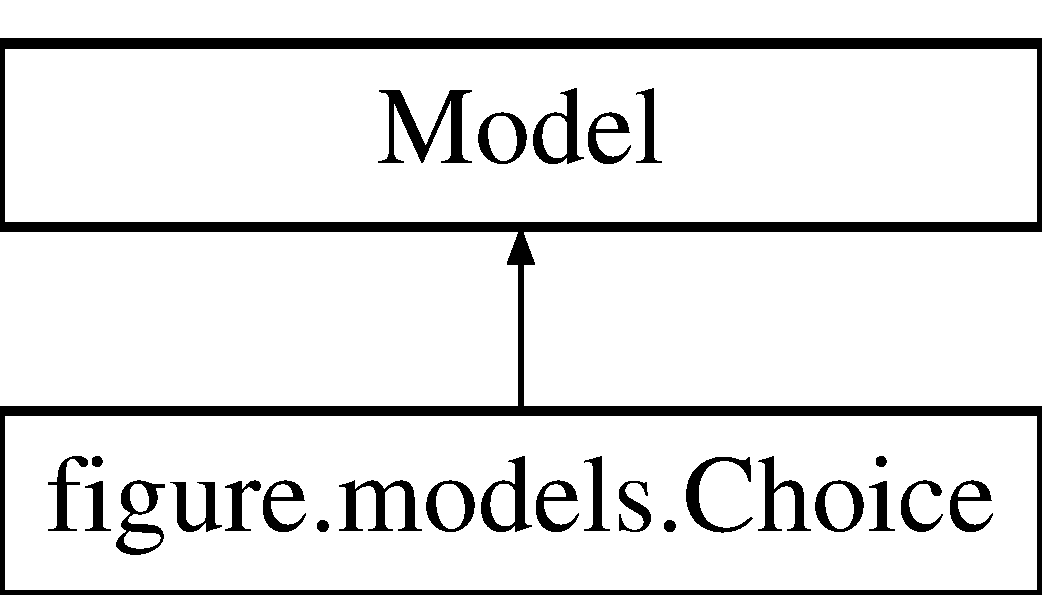
\includegraphics[height=2.000000cm]{classfigure_1_1models_1_1Choice}
\end{center}
\end{figure}
\subsection*{Static Public Attributes}
\begin{DoxyCompactItemize}
\item 
\hypertarget{classfigure_1_1models_1_1Choice_ab56eaa9f5c16b7ca7b02cf249853e12b}{tuple {\bfseries question} = models.\-Foreign\-Key(\hyperlink{classfigure_1_1models_1_1Usage}{Usage})}\label{classfigure_1_1models_1_1Choice_ab56eaa9f5c16b7ca7b02cf249853e12b}

\end{DoxyCompactItemize}


The documentation for this class was generated from the following file\-:\begin{DoxyCompactItemize}
\item 
E\-N\-V/bin/site/mysite/figure/models.\-py\end{DoxyCompactItemize}

\hypertarget{classfigure_1_1models_1_1Usage}{\section{figure.\-models.\-Usage Class Reference}
\label{classfigure_1_1models_1_1Usage}\index{figure.\-models.\-Usage@{figure.\-models.\-Usage}}
}
Inheritance diagram for figure.\-models.\-Usage\-:\begin{figure}[H]
\begin{center}
\leavevmode
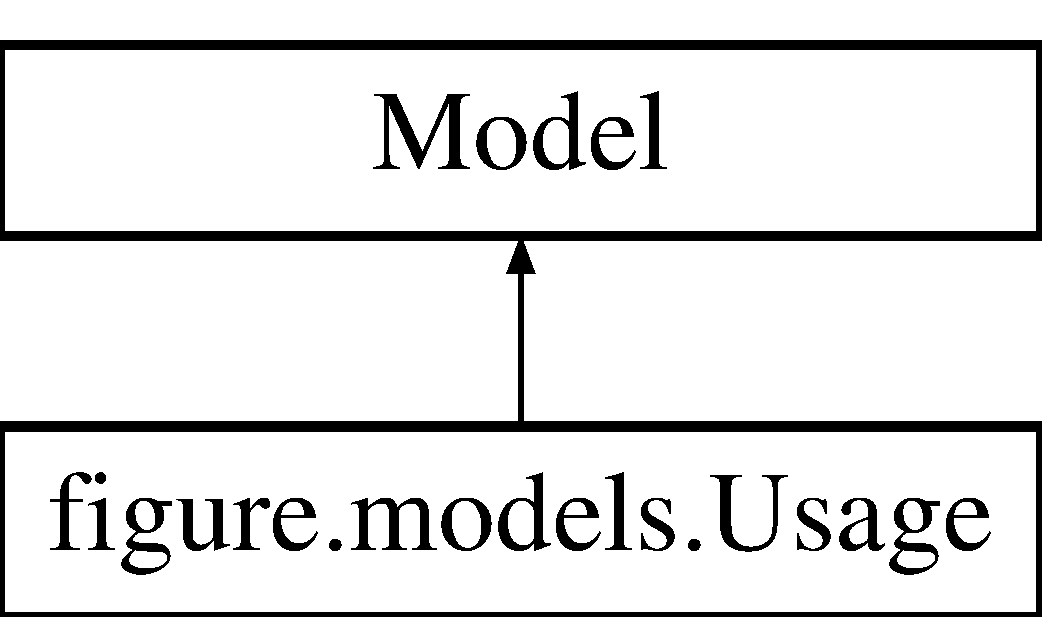
\includegraphics[height=2.000000cm]{classfigure_1_1models_1_1Usage}
\end{center}
\end{figure}
\subsection*{Static Public Attributes}
\begin{DoxyCompactItemize}
\item 
\hypertarget{classfigure_1_1models_1_1Usage_a2d464c09f55e5e5b070fa99db516c6f8}{tuple {\bfseries device\-\_\-usage} = models.\-Integer\-Field(default=0)}\label{classfigure_1_1models_1_1Usage_a2d464c09f55e5e5b070fa99db516c6f8}

\item 
\hypertarget{classfigure_1_1models_1_1Usage_a2390a648c52d4f0f98826581cea8963c}{tuple {\bfseries time\-\_\-stamp} = models.\-Date\-Time\-Field('time recorded')}\label{classfigure_1_1models_1_1Usage_a2390a648c52d4f0f98826581cea8963c}

\end{DoxyCompactItemize}


\subsection{Detailed Description}

\begin{DoxyParams}{Parameters}
{\em models.\-Model} & Take a Django library\\
\hline
\end{DoxyParams}
Two entry fields, one for the timestamp and another for the corresponding usage 

The documentation for this class was generated from the following file\-:\begin{DoxyCompactItemize}
\item 
E\-N\-V/bin/site/mysite/figure/models.\-py\end{DoxyCompactItemize}

\hypertarget{classfigure_1_1tests_1_1UsageTestCase}{\section{figure.\-tests.\-Usage\-Test\-Case Class Reference}
\label{classfigure_1_1tests_1_1UsageTestCase}\index{figure.\-tests.\-Usage\-Test\-Case@{figure.\-tests.\-Usage\-Test\-Case}}
}
Inheritance diagram for figure.\-tests.\-Usage\-Test\-Case\-:\begin{figure}[H]
\begin{center}
\leavevmode
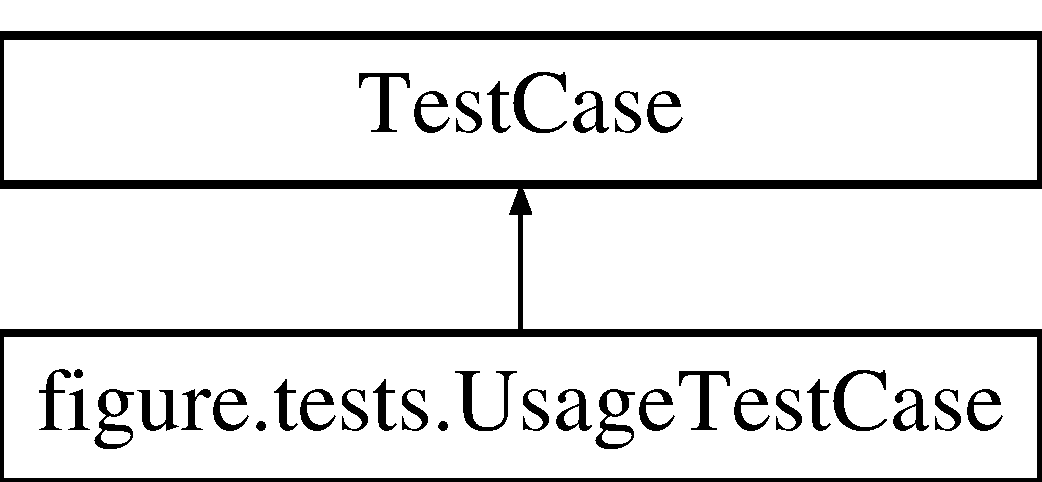
\includegraphics[height=2.000000cm]{classfigure_1_1tests_1_1UsageTestCase}
\end{center}
\end{figure}
\subsection*{Public Member Functions}
\begin{DoxyCompactItemize}
\item 
\hypertarget{classfigure_1_1tests_1_1UsageTestCase_aea573172c8adea7c9350c494fab990d0}{def {\bfseries set\-Up}}\label{classfigure_1_1tests_1_1UsageTestCase_aea573172c8adea7c9350c494fab990d0}

\item 
\hypertarget{classfigure_1_1tests_1_1UsageTestCase_a22b29774c4bccde7385957207932eeef}{def {\bfseries test\-\_\-entry}}\label{classfigure_1_1tests_1_1UsageTestCase_a22b29774c4bccde7385957207932eeef}

\end{DoxyCompactItemize}
\subsection*{Public Attributes}
\begin{DoxyCompactItemize}
\item 
\hypertarget{classfigure_1_1tests_1_1UsageTestCase_a5f98717de545f3b5302a2aef59ccd384}{{\bfseries entry}}\label{classfigure_1_1tests_1_1UsageTestCase_a5f98717de545f3b5302a2aef59ccd384}

\end{DoxyCompactItemize}


The documentation for this class was generated from the following file\-:\begin{DoxyCompactItemize}
\item 
E\-N\-V/bin/site/mysite/figure/tests.\-py\end{DoxyCompactItemize}

\chapter{File Documentation}
\hypertarget{create__db_8py}{\section{server/create\-\_\-db.py File Reference}
\label{create__db_8py}\index{server/create\-\_\-db.\-py@{server/create\-\_\-db.\-py}}
}


Script to create an empty outletify power usage table.  




\subsection{Detailed Description}
Script to create an empty outletify power usage table. 
\hypertarget{dump__test__db_8py}{\section{server/dump\-\_\-test\-\_\-db.py File Reference}
\label{dump__test__db_8py}\index{server/dump\-\_\-test\-\_\-db.\-py@{server/dump\-\_\-test\-\_\-db.\-py}}
}


Script to print out the contents of 'outletify.\-db'.  


\subsection*{Variables}
\begin{DoxyCompactItemize}
\item 
\hypertarget{namespacedump__test__db_ad3fca2acfe4446bb5a67341cc514daef}{tuple {\bfseries dump\-\_\-test\-\_\-db.\-con} = lite.\-connect('outletify.\-db')}\label{namespacedump__test__db_ad3fca2acfe4446bb5a67341cc514daef}

\item 
\hypertarget{namespacedump__test__db_afa8989c3218f5abf8efcb08454a3b8ce}{tuple {\bfseries dump\-\_\-test\-\_\-db.\-cur} = con.\-cursor()}\label{namespacedump__test__db_afa8989c3218f5abf8efcb08454a3b8ce}

\item 
\hypertarget{namespacedump__test__db_adc881780bd64d6e9c8cc8b92211c3d8e}{tuple {\bfseries dump\-\_\-test\-\_\-db.\-rows} = cur.\-execute(\char`\"{}S\-E\-L\-E\-C\-T $\ast$ F\-R\-O\-M sqlite\-\_\-master;\char`\"{})}\label{namespacedump__test__db_adc881780bd64d6e9c8cc8b92211c3d8e}

\end{DoxyCompactItemize}


\subsection{Detailed Description}
Script to print out the contents of 'outletify.\-db'. 
\hypertarget{main_8py}{\section{server/main.py File Reference}
\label{main_8py}\index{server/main.\-py@{server/main.\-py}}
}


Contains the entry point for the uwsgi server.  


\subsection*{Functions}
\begin{DoxyCompactItemize}
\item 
def {\bfseries main.\-get\-\_\-cached\-\_\-file}
\item 
def {\bfseries main.\-untemplateify}
\item 
\hypertarget{namespacemain_ac8009446fd26db57e113618d01e73ef8}{def {\bfseries main.\-application}}\label{namespacemain_ac8009446fd26db57e113618d01e73ef8}

\begin{DoxyCompactList}\small\item\em The entry point for the uwsgi server. \end{DoxyCompactList}\end{DoxyCompactItemize}
\subsection*{Variables}
\begin{DoxyCompactItemize}
\item 
\hypertarget{namespacemain_a210019b4be3192d3347a28bc74fd3dc4}{dictionary {\bfseries main.\-cached\-\_\-files} = \{\}}\label{namespacemain_a210019b4be3192d3347a28bc74fd3dc4}

\end{DoxyCompactItemize}


\subsection{Detailed Description}
Contains the entry point for the uwsgi server. 
\hypertarget{populate__test__db_8py}{\section{server/populate\-\_\-test\-\_\-db.py File Reference}
\label{populate__test__db_8py}\index{server/populate\-\_\-test\-\_\-db.\-py@{server/populate\-\_\-test\-\_\-db.\-py}}
}


Script to add some random data to an Outletify database.  


\subsection*{Variables}
\begin{DoxyCompactItemize}
\item 
\hypertarget{namespacepopulate__test__db_a582308aedcfa0abdb103b8375431fac6}{tuple {\bfseries populate\-\_\-test\-\_\-db.\-dbhandle} = db.\-connect()}\label{namespacepopulate__test__db_a582308aedcfa0abdb103b8375431fac6}

\end{DoxyCompactItemize}


\subsection{Detailed Description}
Script to add some random data to an Outletify database. 
%--- End generated contents ---

% Index
\newpage
\phantomsection
\addcontentsline{toc}{chapter}{Index}
\printindex

\end{document}
